% Source: backpropagation_guide.tex
\begin{notechapter}
% ---- chapter-local definitions ----
\definecolor{nodecolor}{RGB}{70,130,180}
\definecolor{edgecolor}{RGB}{100,100,100}
\definecolor{gradcolor}{RGB}{220,20,60}
\definecolor{examplecolor}{RGB}{240,248,255}
% -----------------------------------
\chapter{Backpropagation as Dynamic Programming}\label{ch:backprop-dynamic-programming}
\chaptersubtitle{Computational graphs and reverse-mode differentiation}

\begin{abstract}
This document provides a clear, example-driven explanation of the backpropagation
algorithm as a dynamic programming method for computing gradients in computational graphs.
We demystify the notation, present the algorithm in both scalar and vector forms,
and show how this fundamental technique enables modern machine learning.
\end{abstract}

\section{Introduction and Motivation}

\subsection{Why Backpropagation Matters}

In machine learning, we need to optimize loss functions that depend on many parameters (often millions).
The fundamental challenge is:

\begin{tcolorbox}[colback=examplecolor,colframe=nodecolor,title=The Core Problem]
Given a complex function $L(\mathbf{w})$ that depends on parameters $\mathbf{w} = [w_1, w_2, \ldots, w_n]$,
we need to compute:
$$\nabla_{\mathbf{w}} L = \left[\frac{\partial L}{\partial w_1},
\frac{\partial L}{\partial w_2}, \ldots, \frac{\partial L}{\partial w_n}\right]$$
to perform gradient descent: $\mathbf{w} \leftarrow \mathbf{w} - \alpha \nabla_{\mathbf{w}} L$
\end{tcolorbox}

\textbf{The difficulty:} In neural networks, the loss function is a deeply nested composition:
$$L = f_k(f_{k-1}(\cdots f_2(f_1(\mathbf{x}; \mathbf{w}_1); \mathbf{w}_2) \cdots; \mathbf{w}_{k-1}); \mathbf{w}_k)$$

Computing gradients naively would require:
\begin{itemize}
    \item Expressing $L$ in closed form (exponentially complex)
    \item Differentiating enormous expressions (computationally infeasible)
    \item Repeating derivative computations (wasteful)
\end{itemize}

\textbf{Backpropagation solves this} by computing all gradients in one backward pass through the computational graph using dynamic programming.

\subsection{Computational Graphs}

\begin{definition}[Computational Graph]
A computational graph is a directed acyclic graph (DAG) where:
\begin{itemize}
    \item Each \textbf{node} $i$ stores a variable $y(i)$
    \item Each \textbf{edge} $(i,j)$ represents that $y(j)$ depends on $y(i)$
    \item Each node computes: $y(j) = f_j(y(i_1), y(i_2), \ldots, y(i_k))$ where $i_1, \ldots, i_k$ are its inputs
\end{itemize}
\end{definition}

\begin{center}
\begin{tikzpicture}[
    node/.style={circle,draw=nodecolor,fill=nodecolor!20,minimum size=1cm,thick},
    edge/.style={->,>=stealth,thick,edgecolor},
    label/.style={font=\small}
]
    % Nodes
    \node[node] (x) at (0,0) {$x$};
    \node[node] (y1) at (2,1) {$y_1$};
    \node[node] (y2) at (2,-1) {$y_2$};
    \node[node] (z) at (4,0) {$z$};
    
    % Edges
    \draw[edge] (x) -- (y1) node[midway,above,sloped,label] {$g_1$};
    \draw[edge] (x) -- (y2) node[midway,below,sloped,label] {$g_2$};
    \draw[edge] (y1) -- (z) node[midway,above,sloped,label] {$f_1$};
    \draw[edge] (y2) -- (z) node[midway,below,sloped,label] {$f_2$};
    
    % Function annotations
    \node[below=0.05cm of x,label] {input};
    \node[above=0.05cm of y1,label] {$y_1=g_1(x)$};
    \node[below=0.05cm of y2,label] {$y_2=g_2(x)$};
    \node[right=0.1cm of z,label] {$z=f(y_1,y_2)$};
\end{tikzpicture}
\end{center}

\section{The Backpropagation Algorithm}

\subsection{Key Notation}

Before presenting the algorithm, let's clarify the notation that often causes confusion:

\begin{tcolorbox}[colback=yellow!10,colframe=orange,title=Essential Notation]
\begin{itemize}
    \item $y(i)$ = the \textbf{value} stored in node $i$
    \item $\mathbf{A}(i)$ = the set of nodes that $i$ \textbf{points to} (node $i$'s children/successors)
    \item $z(i,j) = \frac{\partial y(j)}{\partial y(i)}$ = \textbf{local derivative} on edge $(i,j)$
    \item $S(i,t) = \frac{\partial y(t)}{\partial y(i)}$ = derivative of output $t$ w.r.t. node $i$
    \item $L$ = loss function (computed at output node)
    \item $\Delta(i) = \frac{\partial L}{\partial y(i)}$ = \textbf{gradient} at node $i$ (what we propagate backward)
\end{itemize}
\end{tcolorbox}

\textbf{Example of $\mathbf{A}(i)$:}

\begin{center}
\begin{tikzpicture}[
    node/.style={circle,draw=nodecolor,fill=nodecolor!20,minimum size=0.8cm,thick},
    edge/.style={->,>=stealth,thick,edgecolor}
]
    \node[node] (1) at (0,1) {1};
    \node[node] (2) at (0,-1) {2};
    \node[node] (3) at (2,2) {3};
    \node[node] (4) at (2,0) {4};
    \node[node] (5) at (2,-2) {5};
    \node[node] (6) at (4,0) {6};
    
    \draw[edge] (1) -- (3);
    \draw[edge] (1) -- (4);
    \draw[edge] (2) -- (4);
    \draw[edge] (2) -- (5);
    \draw[edge] (3) -- (6);
    \draw[edge] (4) -- (6);
    \draw[edge] (5) -- (6);
    
    \node[below=0.05cm of 1,font=\small] {$\mathbf{A}(1) = \{3,4\}$};
    \node[below=0.05cm of 2,font=\small] {$\mathbf{A}(2) = \{4,5\}$};
    \node[below=0.05cm of 4,font=\small] {$\mathbf{A}(4) = \{6\}$};
\end{tikzpicture}
\end{center}

\subsection{The Core Algorithm: Node-to-Node Derivatives}

\begin{algorithm}[H]
\caption{Compute Node-to-Node Derivatives (Scalar Version)}
\begin{algorithmic}[1]
\Require Computational graph with nodes, source node $s$, target node $t$
\Ensure $S(s,t) = \frac{\partial y(t)}{\partial y(s)}$
\State \textbf{Forward Pass:} Compute all node values $y(i)$ from inputs to outputs
\State \textbf{Compute Local Derivatives:} For each edge $(i,j)$, compute $z(i,j) = \frac{\partial y(j)}{\partial y(i)}$
\State \textbf{Initialize:} $S(t,t) \gets 1$ \Comment{Derivative of output w.r.t. itself}
\State \textbf{Create:} Empty queue $Q$, add $t$ to $Q$
\While{$Q$ is not empty}
    \State Remove node $i$ from $Q$
    \For{each node $p$ such that $i \in \mathbf{A}(p)$} \Comment{$p$ points to $i$}
        \If{$S(p,t)$ not yet computed and all nodes in $\mathbf{A}(p)$ are processed}
            \State $S(p,t) \gets \sum_{j \in \mathbf{A}(p)} S(j,t) \cdot z(p,j)$ \Comment{\textbf{Dynamic programming update}}
            \State Add $p$ to $Q$
        \EndIf
    \EndFor
\EndWhile
\State \Return $S(s,t)$
\end{algorithmic}
\end{algorithm}

\begin{tcolorbox}[colback=green!5,colframe=green!60,title=Extension to Multiple Output Nodes]
\textbf{Question:} What if we have multiple output nodes $t_1, t_2, \ldots, t_p$?

\textbf{Answer:} Algorithm 1 computes derivatives for a \textbf{single target} node $t$. For multiple outputs, you have two options:

\textbf{Option 1: Run the algorithm multiple times}
\begin{itemize}
    \item Run Algorithm 1 once for each target $t_r$
    \item Initialize: $S(t_r, t_r) \gets 1$ for the specific target
    \item This gives you $S(s, t_1), S(s, t_2), \ldots, S(s, t_p)$ separately
\end{itemize}

\textbf{Option 2: Compute all targets simultaneously (more efficient)}
\begin{itemize}
    \item Initialize: $S(t_r, t_r) \gets 1$ for \textbf{all} output nodes $t_r$
    \item Add all output nodes to the initial queue: $Q \gets \{t_1, t_2, \ldots, t_p\}$
    \item Maintain separate $S(i, t_r)$ values for each target $t_r$
    \item The update becomes: For each target $t_r$, compute $S(p, t_r) \gets \sum_{j \in \mathbf{A}(p)} S(j, t_r) \cdot z(p,j)$
\end{itemize}

For neural networks with a \textbf{loss function}, we typically have a single scalar output (the loss), so we only need one target. This is what Algorithm 2 handles.
\end{tcolorbox}

\textbf{Key Insight:} Line 9 is the multivariate chain rule:
$$\frac{\partial y(t)}{\partial y(p)} = \sum_{j \in \mathbf{A}(p)} \frac{\partial y(t)}{\partial y(j)} \cdot \frac{\partial y(j)}{\partial y(p)}$$

\begin{tcolorbox}[colback=yellow!5,colframe=orange!80,title=Understanding the IF Condition (Line 8)]
\textbf{Question:} What happens if all nodes in $\mathbf{A}(p)$ are \textbf{NOT} yet processed?

\textbf{Answer:} Node $p$ is simply \textbf{skipped} in this iteration. It will be reconsidered later when we process one of its children. Here's why this works:

\begin{enumerate}
    \item The algorithm processes nodes in a \textbf{queue}
    \item When we process node $i$, we look at all its \textbf{parents} (nodes $p$ where $i \in \mathbf{A}(p)$)
    \item Each parent $p$ can only be computed when \textbf{all} its children are ready
    \item If not all children are ready, we skip $p$ now
    \item When we later process another child of $p$, we check $p$ again
    \item Eventually all children of $p$ will be processed, and then $p$ gets computed
\end{enumerate}

\textbf{Key property:} In a DAG, this process always terminates because there are no cycles. Every node will eventually have all its children processed.
\end{tcolorbox}

\subsection{Complete Trace of Algorithm 1 on Example Graph}

Let's trace Algorithm 1 step-by-step on the example graph from Section 2.1, computing $S(1,6) = \frac{\partial y(6)}{\partial y(1)}$.

\textbf{Recall the graph:}
\begin{center}
\begin{tikzpicture}[
    node/.style={circle,draw=nodecolor,fill=nodecolor!20,minimum size=0.8cm,thick},
    edge/.style={->,>=stealth,thick,edgecolor}
]
    \node[node] (1) at (0,1) {1};
    \node[node] (2) at (0,-1) {2};
    \node[node] (3) at (2,2) {3};
    \node[node] (4) at (2,0) {4};
    \node[node] (5) at (2,-2) {5};
    \node[node] (6) at (4,0) {6};
    
    \draw[edge] (1) -- (3);
    \draw[edge] (1) -- (4);
    \draw[edge] (2) -- (4);
    \draw[edge] (2) -- (5);
    \draw[edge] (3) -- (6);
    \draw[edge] (4) -- (6);
    \draw[edge] (5) -- (6);
    
    \node[below=0.05cm of 1,font=\footnotesize] {$\mathbf{A}(1) = \{3,4\}$};
    \node[below=0.05cm of 2,font=\footnotesize] {$\mathbf{A}(2) = \{4,5\}$};
    \node[below=0.05cm of 3,font=\footnotesize] {$\mathbf{A}(3) = \{6\}$};
    \node[below=0.05cm of 4,font=\footnotesize] {$\mathbf{A}(4) = \{6\}$};
    \node[below=0.05cm of 5,font=\footnotesize] {$\mathbf{A}(5) = \{6\}$};
\end{tikzpicture}
\end{center}

\textbf{Setup:} Source $s=1$, Target $t=6$. Assume all local derivatives $z(i,j)$ are already computed.

\begin{tcolorbox}[colback=blue!5,colframe=blue!60,title=Initialization]
\textbf{Lines 3-4:}
\begin{itemize}
    \item $S(6,6) \gets 1$
    \item $Q \gets \{6\}$
    \item Processed: $\{6\}$
\end{itemize}
\end{tcolorbox}

\begin{tcolorbox}[
    colback=blue!5,
    colframe=blue!60,
    title=Iteration 1: Process Node 6,
    sidebyside,
    sidebyside align=top seam, % Aligns the absolute tops of both sides
    righthand width=4.5cm,
    sidebyside gap=5mm
    ]
Line 7: Find parents of 6 (nodes $p$ where $6 \in \mathbf{A}(p)$): Parents are $\{3, 4, 5\}$

\begin{minipage}[t]{\linewidth}
Check each parent:
\begin{itemize}
    \item \textbf{Node 3:} $\mathbf{A}(3) = \{6\}$.\\
    All children processed? \textcolor{green!60!black}{Yes} (6 is processed)
    
    Compute: $S(3,6) = S(6,6) \cdot z(3,6) = z(3,6)$
    \vspace{0.3em}\\
    Add 3 to $Q$
    
    \item \textbf{Node 4:} $\mathbf{A}(4) = \{6\}$.\\
    All children processed? \textcolor{green!60!black}{Yes}
    
    Compute: $S(4,6) = z(4,6)$
    \vspace{0.3em}\\
    Add 4 to $Q$
    
    \item \textbf{Node 5:} $\mathbf{A}(5) = \{6\}$.\\
    All children processed? \textcolor{green!60!black}{Yes}
    
    Compute: $S(5,6) = z(5,6)$
    \vspace{0.3em}\\
    Add 5 to $Q$
\end{itemize}
\end{minipage}
\vspace{0.5em}

\textbf{After iteration 1:} $Q = \{3, 4, 5\}$, Processed: $\{6, 3, 4, 5\}$

\tcblower % Divider to the right side

\begin{tikzpicture}[
    baseline=(current bounding box.north),
    node/.style={circle,draw=nodecolor,fill=nodecolor!20,minimum size=0.8cm,thick},
    edge/.style={->,>=stealth,thick,edgecolor}
]
    \node[node] (3) at (2,2) {3};
    \node[node] (4) at (2,0) {4};
    \node[node] (5) at (2,-2) {5};
    \node[node] (6) at (4,0) {\textbf{6}};
    
    \draw[edge] (3) -- (6);
    \draw[edge] (4) -- (6);
    \draw[edge] (5) -- (6);
 
    \node[below=0.05cm of 3,font=\footnotesize] {$\mathbf{A}(3) = \{\mathbf{6}\}$};
    \node[below=0.05cm of 4,font=\footnotesize] {$\mathbf{A}(4) = \{\mathbf{6}\}$};
    \node[below=0.05cm of 5,font=\footnotesize] {$\mathbf{A}(5) = \{\mathbf{6}\}$};
\end{tikzpicture}
\end{tcolorbox}

\begin{tcolorbox}[
    colback=blue!5,
    colframe=blue!60,
    title=Iteration 2: Process Node 3,
    sidebyside,
    sidebyside align=top seam, % Aligns the absolute tops of both sides
    righthand width=4.5cm,
    sidebyside gap=5mm]

Line 7: Find parents of 3 (nodes $p$ where $3 \in \mathbf{A}(p)$): Parent is $\{1\}$

\begin{minipage}[t]{\linewidth}
Check node 1:
\begin{itemize}
    \item \textbf{Node 1:} $\mathbf{A}(1) = \{3, 4\}$. All children processed?
    
    Node 3? \textcolor{green!60!black}{Yes} \quad Node 4? \textcolor{green!60!black}{Yes} (processed in iteration 1)
    
    Compute: $S(1,6) = S(3,6) \cdot z(1,3) + S(4,6) \cdot z(1,4)$
    
    $\boxed{S(1,6) = z(3,6) \cdot z(1,3) + z(4,6) \cdot z(1,4)}$
    \vspace{0.5em}\\
    Add 1 to $Q$
\end{itemize}
\end{minipage}
\vspace{0.5em}

\textbf{After iteration 2:} $Q = \{4, 5, 1\}$, Processed: $\{6, 3, 4, 5, 1\}$

\tcblower % Divider to the right side

\begin{tikzpicture}[
    baseline=(current bounding box.north),
    node/.style={circle,draw=nodecolor,fill=nodecolor!20,minimum size=0.8cm,thick},
    edge/.style={->,>=stealth,thick,edgecolor}
]
    \node[node] (1) at (0,1) {1};
    \node[node] (3) at (2,2) {\textbf{3}};
    \node[node] (4) at (2,0) {4};
    \node[node] (6) at (4,0) {6};
    
    \draw[edge] (1) -- (3);
    \draw[edge] (1) -- (4);
    \draw[edge] (3) -- (6);
    \draw[edge] (4) -- (6);
    
    \node[right=0.05cm of 1,font=\footnotesize] {$\mathbf{A}(1) = \{\mathbf{3},4\}$};
    \node[above=0.05cm of 3,font=\footnotesize] {$\mathbf{A}(3) = \{6\}$};
    \node[below=0.05cm of 4,font=\footnotesize] {$\mathbf{A}(4) = \{6\}$};
\end{tikzpicture}
\end{tcolorbox}

\begin{tcolorbox}[
    colback=blue!5,
    colframe=blue!60,
    title=Iteration 3: Process Node 4,
    sidebyside,
    sidebyside align=top seam, % Aligns the absolute tops of both sides
    righthand width=4.5cm,
    sidebyside gap=5mm]

Line 7: Find parents of 4 (nodes $p$ where $4 \in \mathbf{A}(p)$): Parents are $\{1, 2\}$

\begin{minipage}[t]{\linewidth}
Check each parent:
\begin{itemize}
    \item \textbf{Node 1:} Already computed in iteration 2, \textcolor{orange}{skip}
    
    \item \textbf{Node 2:} $\mathbf{A}(2) = \{4, 5\}$. All children processed?
    
    Node 4? \textcolor{green!60!black}{Yes} \quad Node 5? \textcolor{green!60!black}{Yes}
    
    Compute: $S(2,6) = S(4,6) \cdot z(2,4) + S(5,6) \cdot z(2,5)$
    
    Add 2 to $Q$
\end{itemize}
\end{minipage}
\vspace{0.5em}

\textbf{After iteration 3:} $Q = \{5, 1, 2\}$, Processed: $\{6, 3, 4, 5, 1, 2\}$

\tcblower % Divider to the right side

\begin{tikzpicture}[
    baseline=(current bounding box.north),
    node/.style={circle,draw=nodecolor,fill=nodecolor!20,minimum size=0.8cm,thick},
    edge/.style={->,>=stealth,thick,edgecolor}
]
    \node[node] (1) at (0,1.5) {1};
    \node[node] (2) at (0,-1) {2};
    \node[node] (4) at (2,0) {\textbf{4}};
    \node[node] (5) at (2,-2) {5};
    \node[node] (6) at (4,0) {6};
    
    \draw[edge] (1) -- (4);
    \draw[edge] (2) -- (4);
    \draw[edge] (2) -- (5);
    \draw[edge] (4) -- (6);
    \draw[edge] (5) -- (6);
    
    \node[right=0.05cm of 1,font=\footnotesize] {$\mathbf{A}(1) = \{3,\mathbf{4}\}$};
    \node[right=0.05cm of 2,font=\footnotesize] {$\mathbf{A}(2) = \{\mathbf{4},5\}$};
    \node[above=-0.1cm of 4,font=\footnotesize] {$\mathbf{A}(4) = \{6\}$};
    \node[below=0.05cm of 5,font=\footnotesize] {$\mathbf{A}(5) = \{6\}$};
\end{tikzpicture}
\end{tcolorbox}

\begin{tcolorbox}[colback=blue!5,colframe=blue!60,title=Iterations 4-6: Cleanup]
\textbf{Iteration 4:} Process node 5. Parent is node 2, already computed. \textcolor{orange}{Skip}.

\textbf{Iterations 5-6:} Process nodes 1 and 2. Both already computed, no parents to update.

\textbf{Result:} Queue $Q = \{\}$ (empty). \textbf{Algorithm terminates.}

\textbf{Return:} $\boxed{S(1,6) = z(3,6) \cdot z(1,3) + z(4,6) \cdot z(1,4)}$
\end{tcolorbox}

\textbf{Key Observations:}
\begin{enumerate}
    \item Node 1 could only be computed after \textbf{both} nodes 3 and 4 were processed
    \item Node 2 could only be computed after \textbf{both} nodes 4 and 5 were processed
    \item The order matters! We process in reverse topological order (from output to input)
    \item The final result is: $S(1,6) = z(3,6) \cdot z(1,3) + z(4,6) \cdot z(1,4)$
    \item This represents the sum over the two paths from node 1 to node 6
\end{enumerate}

\subsection{The Full Algorithm: Loss-to-Weight Derivatives}

For machine learning, we need derivatives of the loss $L$ with respect to weights, not just node-to-node derivatives.

\subsubsection{Understanding the Relationship}

\begin{tcolorbox}[colback=examplecolor,colframe=nodecolor,title=Key Insight: From Node-to-Node to Loss-to-Weight]
The loss-to-weight derivative computation has two steps:

\textbf{Step 1:} Compute loss-to-node derivatives $\Delta(i) = \frac{\partial L}{\partial y(i)}$ for all nodes $i$

This is essentially the same as the node-to-node algorithm, but:
\begin{itemize}
    \item Instead of initializing $S(t,t) = 1$, we initialize $\Delta(t) = \frac{\partial L}{\partial y(t)}$ at output nodes
    \item We propagate the \textbf{loss gradient} backward instead of just derivatives
\end{itemize}

\textbf{Step 2:} Convert node gradients to weight gradients using the chain rule

For a weight $w_{ji}$ on edge $(j,i)$:
$$\frac{\partial L}{\partial w_{ji}} = \frac{\partial L}{\partial y(i)} \cdot \frac{\partial y(i)}{\partial w_{ji}} = \Delta(i) \cdot \frac{\partial y(i)}{\partial w_{ji}}$$
\end{tcolorbox}

\subsubsection{Why Node-to-Node is a Special Case}

Think about it this way: In the node-to-node algorithm, we computed $S(i,t) = \frac{\partial y(t)}{\partial y(i)}$. This is asking: "How does the output node $t$ change when node $i$ changes?"

In the loss-to-weight algorithm, we compute $\Delta(i) = \frac{\partial L}{\partial y(i)}$. This is asking: "How does the loss $L$ change when node $i$ changes?"

\textbf{The key realization:} The loss $L$ is just a special node that we compute from the output nodes! So:
\begin{itemize}
    \item Node-to-node: $\frac{\partial y(\text{target node})}{\partial y(i)}$
    \item Loss-to-node: $\frac{\partial L(\text{function of output nodes})}{\partial y(i)}$
\end{itemize}

They use the same dynamic programming structure, just with different initialization!

\subsubsection{Detailed Algorithm Breakdown}

\begin{algorithm}[H]
\caption{Backpropagation for Loss-to-Weight Derivatives (Detailed)}
\begin{algorithmic}[1]
\Require Computational graph, loss function $L$, output node(s) $t_1, \ldots, t_p$
\Ensure $\frac{\partial L}{\partial w_{ji}}$ for all weights $w_{ji}$
\State \textbf{Forward Pass:} Compute all node values from inputs to outputs
\State \textbf{Compute Local Derivatives:} For each edge $(i,j)$, compute $z(i,j) = \frac{\partial y(j)}{\partial y(i)}$
\State \textbf{Initialize:} For each output node $t_r$: $\Delta(t_r) \gets \frac{\partial L}{\partial y(t_r)}$ \Comment{Loss derivative at outputs}
\State \textbf{Create:} Empty set of processed nodes $P \gets \{t_1, \ldots, t_p\}$
\For{each node $i$ in reverse topological order (output to input)} \Comment{Visit nodes backward}
    \If{$i$ is an output node}
        \State Skip (already initialized) \Comment{$\Delta(i)$ already set}
    \Else
        \State $\Delta(i) \gets \sum_{j \in \mathbf{A}(i)} \Delta(j) \cdot z(i,j)$ \Comment{Backpropagate: same as node-to-node!}
    \EndIf
\EndFor
\State \textbf{Compute Weight Gradients:}
\For{each edge $(j,i)$ with weight $w_{ji}$}
    \State $\frac{\partial L}{\partial w_{ji}} \gets \Delta(i) \cdot \frac{\partial y(i)}{\partial w_{ji}}$ \Comment{Chain rule: loss-to-node $\times$ node-to-weight}
\EndFor
\State \Return All weight gradients $\left\{\frac{\partial L}{\partial w_{ji}}\right\}$
\end{algorithmic}
\end{algorithm}

\subsubsection{Visualizing the Two-Step Process}

Consider a simple network where nodes compute arbitrary functions:

\begin{center}
\begin{tikzpicture}[
    node/.style={circle,draw=nodecolor,fill=nodecolor!20,minimum size=1cm,thick},
    edge/.style={->,>=stealth,thick,edgecolor},
    weight/.style={font=\small,red!70!black},
    grad/.style={font=\small,blue!70!black}
]
    \node[node] (x) at (0,0) {$x$};
    \node[node] (y1) at (2,1) {$y_1$};
    \node[node] (y2) at (2,-1) {$y_2$};
    \node[node] (o) at (4,0) {$o$};
    \node[node] (L) at (6,0) {$L$};
    
    \draw[edge] (x) -- (y1) node[midway,above,sloped,weight] {$f_1$};
    \draw[edge] (x) -- (y2) node[midway,below,sloped,weight] {$f_2$};
    \draw[edge] (y1) -- (o) node[midway,above,sloped,weight] {$g_1$};
    \draw[edge] (y2) -- (o) node[midway,below,sloped,weight] {$g_2$};
    \draw[edge] (o) -- (L) node[midway,above] {loss};
    
    \node[below=0.3cm of x] {Input};
    \node[above=0.1cm of y1,font=\footnotesize] {$y_1 = f_1(x; w_1)$};
    \node[below=0.1cm of y2,font=\footnotesize] {$y_2 = f_2(x; w_2)$};
    \node[above=0.3cm of o,font=\footnotesize] {$o = g(y_1, y_2; w_3, w_4)$};
    \node[below=0.3cm of L] {$L = \ell(o, y_{\text{true}})$};
\end{tikzpicture}
\end{center}

Here $f_1, f_2, g$ are \textbf{arbitrary differentiable functions} with parameters (weights). They could be:
\begin{itemize}
    \item Linear: $f_1(x; w_1) = w_1 x$
    \item Nonlinear with activation: $f_1(x; w_1) = \tanh(w_1 x)$
    \item Multivariate: $g(y_1, y_2; w_3, w_4) = w_3 y_1 + w_4 y_2$ or $g(y_1, y_2; w_3, w_4) = w_3 \sigma(y_1) + w_4 y_2^2$
    \item Any differentiable function!
\end{itemize}

\textbf{The key requirement:} We must be able to compute $\frac{\partial y(j)}{\partial y(i)}$ (node-to-node) and $\frac{\partial y(i)}{\partial w}$ (node-to-weight) for each function.

\textbf{Step 1: Compute loss-to-node derivatives (backward pass)}

\begin{center}
\begin{tikzpicture}[
    node/.style={circle, draw=blue!80, fill=blue!5, minimum size=1cm, thick},
    % Backprop edges: Red, dashed, with larger arrowheads
    edge/.style={<-, >={Stealth[scale=1.2]}, thick, red!80!black, dashed},
    label_edge/.style={font=\scriptsize, sloped, midway},
    label_node/.style={font=\footnotesize, color=red!90!black, font=\bfseries}
]
    % 1. Nodes with increased horizontal distance (3.5 units)
    \node[node] (x) at (0,0) {$x$};
    \node[node] (y1) at (3.5, 1.2) {$y_1$};
    \node[node] (y2) at (3.5, -1.2) {$y_2$};
    \node[node] (o) at (7,0) {$o$};
    \node[node] (L) at (9.5,0) {$L$};
    
    % 2. Backward Edges (Chain Rule visualization)
    % Labels moved slightly with yshift to avoid sitting exactly on the dashed line
    \draw[edge] (x) -- (y1) node[label_edge, above, yshift=2pt] {$\Delta(y_1) \cdot \frac{\partial y_1}{\partial x}$};
    \draw[edge] (x) -- (y2) node[label_edge, below, yshift=-2pt] {$\Delta(y_2) \cdot \frac{\partial y_2}{\partial x}$};
    
    \draw[edge] (y1) -- (o) node[label_edge, above, yshift=2pt] {$\Delta(o) \cdot \frac{\partial o}{\partial y_1}$};
    \draw[edge] (y2) -- (o) node[label_edge, below, yshift=-2pt] {$\Delta(o) \cdot \frac{\partial o}{\partial y_2}$};
    
    \draw[edge] (o) -- (L) node[midway, above, font=\scriptsize, yshift=2pt] {$\frac{\partial L}{\partial o}$};
    
    % 3. Delta values at nodes (The "messages" being passed)
    \node[above right=0.1cm of L, label_node] {$\Delta(L) = 1$};
    \node[above=0.1cm of o, label_node] {$\Delta(o)$};
    \node[above=0.1cm of y1, label_node] {$\Delta(y_1)$};
    \node[below=0.1cm of y2, label_node] {$\Delta(y_2)$};
    \node[left=0.1cm of x, label_node] {$\Delta(x)$};

    % 4. Legend / Annotation
    \node[below=1.8cm of o, font=\scriptsize, draw, dashed, inner sep=5pt] {
        \begin{tabular}{l}
            \textbf{Backpropagation Rule:}\\
            $\Delta(\text{input}) = \Delta(\text{output}) \cdot \frac{\partial \text{output}}{\partial \text{input}}$
        \end{tabular}
    };

\end{tikzpicture}
\end{center}

\textbf{Step 2: Convert to weight gradients}

For each weight, multiply the node gradient by the local derivative. The specific form of $\frac{\partial y(i)}{\partial w}$ depends on how node $i$ uses weight $w$:

\textbf{General formula:}
\begin{align*}
\frac{\partial L}{\partial w_1} &= \Delta(y_1) \cdot \frac{\partial y_1}{\partial w_1} = \Delta(y_1) \cdot \frac{\partial f_1(x; w_1)}{\partial w_1}\\
\frac{\partial L}{\partial w_2} &= \Delta(y_2) \cdot \frac{\partial y_2}{\partial w_2} = \Delta(y_2) \cdot \frac{\partial f_2(x; w_2)}{\partial w_2}\\
\frac{\partial L}{\partial w_3} &= \Delta(o) \cdot \frac{\partial o}{\partial w_3} = \Delta(o) \cdot \frac{\partial g(y_1, y_2; w_3, w_4)}{\partial w_3}\\
\frac{\partial L}{\partial w_4} &= \Delta(o) \cdot \frac{\partial o}{\partial w_4} = \Delta(o) \cdot \frac{\partial g(y_1, y_2; w_3, w_4)}{\partial w_4}
\end{align*}

\textbf{For the linear case specifically} ($y_1 = w_1 x$, $y_2 = w_2 x$, $o = w_3 y_1 + w_4 y_2$):
\begin{align*}
\frac{\partial L}{\partial w_1} &= \Delta(y_1) \cdot x\\
\frac{\partial L}{\partial w_2} &= \Delta(y_2) \cdot x\\
\frac{\partial L}{\partial w_3} &= \Delta(o) \cdot y_1\\
\frac{\partial L}{\partial w_4} &= \Delta(o) \cdot y_2
\end{align*}

\subsubsection{Complete Numerical Example}

Let's work through a concrete example. \textbf{For simplicity}, we'll use linear functions, but remember that the algorithm works for \textbf{any} differentiable functions!

\begin{example}[Loss-to-Weight Computation with Linear Functions]
Consider a network where:
\begin{itemize}
    \item $y_1 = f_1(x; w_1) = w_1 \cdot x$ (linear function)
    \item $y_2 = f_2(x; w_2) = w_2 \cdot x$ (linear function)
    \item $o = g(y_1, y_2; w_3, w_4) = w_3 y_1 + w_4 y_2$ (linear combination)
    \item $L = \frac{1}{2}(o - y_{\text{true}})^2$ (MSE loss)
\end{itemize}

With values:
\begin{itemize}
    \item Input: $x = 2$
    \item Weights: $w_1 = 0.5, w_2 = -0.3, w_3 = 1.2, w_4 = 0.8$
    \item True output: $y_{\text{true}} = 1.0$
\end{itemize}
\end{example}

\begin{tcolorbox}[
    colback=blue!5,
    colframe=blue!60,
    title=Step 1: Forward Pass,
    sidebyside,
    sidebyside align=top seam,
    righthand width=6.5cm,
    sidebyside gap=5mm]

Compute all node values:
\begin{align*}
y_1 &= w_1 \cdot x = 0.5 \cdot 2 = 1.0\\
y_2 &= w_2 \cdot x = -0.3 \cdot 2 = -0.6\\
o &= w_3 \cdot y_1 + w_4 \cdot y_2\\
&= 1.2 \cdot 1.0 + 0.8 \cdot (-0.6)\\
&= 1.2 - 0.48 = 0.72\\
L &= \frac{1}{2}(o - y_{\text{true}})^2\\
&= \frac{1}{2}(0.72 - 1.0)^2\\
&= \frac{1}{2}(-0.28)^2 = 0.0392
\end{align*}

\tcblower

\begin{tikzpicture}[
    baseline=(current bounding box.north),
    node/.style={circle,draw=nodecolor,fill=nodecolor!20,minimum size=0.9cm,thick},
    edge/.style={->,>=stealth,thick,edgecolor},
    label/.style={font=\tiny}]
    
    \node[node] (x) at (0,0) {$x$};
    \node[node] (y1) at (2,1.5) {$y_1$};
    \node[node] (y2) at (2,-1.5) {$y_2$};
    \node[node] (o) at (4,0) {$o$};
    \node[node] (L) at (5.8,0) {$L$};
    
    \draw[edge] (x) -- (y1);
    \draw[edge] (x) -- (y2);
    \draw[edge] (y1) -- (o);
    \draw[edge] (y2) -- (o);
    \draw[edge] (o) -- (L);
    
    \node[below=0.1cm of x,label,blue!70!black] {$x=2$};
    \node[above=0.05cm of y1,label,blue!70!black] {$y_1=1.0$};
    \node[below=0.05cm of y2,label,blue!70!black] {$y_2=-0.6$};
    \node[above=0.1cm of o,label,blue!70!black] {$o=0.72$};
    \node[above=0.1cm of L,label,blue!70!black] {$L=0.0392$};
\end{tikzpicture}
\end{tcolorbox}

\begin{tcolorbox}[
    colback=blue!5,
    colframe=blue!60,
    title=Step 2: Compute Local Derivatives,
    sidebyside,
    sidebyside align=top seam,
    righthand width=6.5cm,
    sidebyside gap=5mm]

For each edge, compute $z(i,j) = \frac{\partial y(j)}{\partial y(i)}$:
\begin{align*}
z(x, y_1) &= \frac{\partial y_1}{\partial x} = w_1 = 0.5\\
z(x, y_2) &= \frac{\partial y_2}{\partial x} = w_2 = -0.3\\
z(y_1, o) &= \frac{\partial o}{\partial y_1} = w_3 = 1.2\\
z(y_2, o) &= \frac{\partial o}{\partial y_2} = w_4 = 0.8\\
z(o, L) &= \frac{\partial L}{\partial o}\\
&= o - y_{\text{true}}\\
&= 0.72 - 1.0 = -0.28
\end{align*}

\tcblower

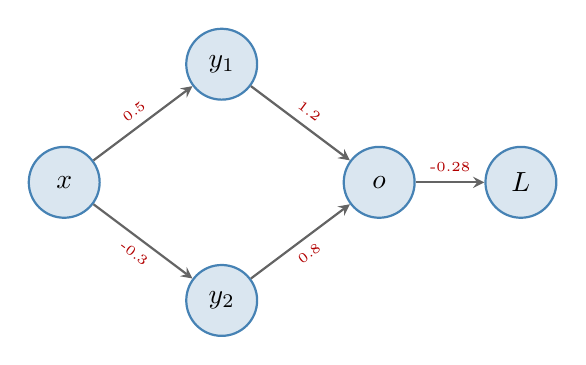
\begin{tikzpicture}[
    baseline=(current bounding box.north),
    node/.style={circle,draw=nodecolor,fill=nodecolor!20,minimum size=0.9cm,thick},
    edge/.style={->,>=stealth,thick,edgecolor},
    label/.style={font=\tiny}]
    
    \node[node] (x) at (0,0) {$x$};
    \node[node] (y1) at (2,1.5) {$y_1$};
    \node[node] (y2) at (2,-1.5) {$y_2$};
    \node[node] (o) at (4,0) {$o$};
    \node[node] (L) at (5.8,0) {$L$};
    
    \draw[edge] (x) -- (y1) node[midway,above,sloped,label,red!70!black] {0.5};
    \draw[edge] (x) -- (y2) node[midway,below,sloped,label,red!70!black] {-0.3};
    \draw[edge] (y1) -- (o) node[midway,above,sloped,label,red!70!black] {1.2};
    \draw[edge] (y2) -- (o) node[midway,below,sloped,label,red!70!black] {0.8};
    \draw[edge] (o) -- (L) node[midway,above,label,red!70!black] {-0.28};

\end{tikzpicture}
\end{tcolorbox}

\begin{tcolorbox}[
    colback=green!5,
    colframe=green!60,
    title=Step 3: Backward Pass (Compute Node Gradients),
    sidebyside,
    sidebyside align=top seam,
    righthand width=6.5cm,
    sidebyside gap=5mm]

\textbf{Initialize at loss:}
$$\Delta(L) = 1$$

\textbf{At output node $o$:}
$$\Delta(o) = z(o, L) = -0.28$$

\textbf{At node $y_1$:}\\
$\mathbf{A}(y_1) = \{o\}$
$$\Delta(y_1) = \Delta(o) \cdot z(y_1, o)$$
$$= -0.28 \cdot 1.2 = -0.336$$

\textbf{At node $y_2$:}\\
$\mathbf{A}(y_2) = \{o\}$
$$\Delta(y_2) = \Delta(o) \cdot z(y_2, o)$$
$$= -0.28 \cdot 0.8 = -0.224$$

\textbf{At input $x$:}\\
$\mathbf{A}(x) = \{y_1, y_2\}$
\begin{align*}
\Delta(x) &= \Delta(y_1) \cdot z(x, y_1)\\
&\quad + \Delta(y_2) \cdot z(x, y_2)\\
&= -0.336 \cdot 0.5\\
&\quad + (-0.224) \cdot (-0.3)\\
&= -0.1008
\end{align*}

\tcblower

\begin{tikzpicture}[
    baseline=(current bounding box.north),
    node/.style={circle,draw=nodecolor,fill=nodecolor!20,minimum size=0.9cm,thick},
    edge/.style={<-,>=stealth,thick,gradcolor,dashed},
    gray_edge/.style={<-,>=stealth,thick,gray,dashed},
    label/.style={font=\tiny}]
    
    \node[node] (x) at (0,0) {$x$};
    \node[node] (y1) at (2,1.5) {$y_1$};
    \node[node] (y2) at (2,-1.5) {$y_2$};
    \node[node] (o) at (4,0) {$o$};
    \node[node] (L) at (5.8,0) {$L$};
    
    \draw[gray_edge] (x) -- (y1) node[midway,above,sloped,label,red!70!black]{};
    \draw[gray_edge] (x) -- (y2) node[midway,below,sloped,label,red!70!black]{};
    \draw[gray_edge] (y1) -- (o) node[midway,above,sloped,label,red!70!black]{};
    \draw[gray_edge] (y2) -- (o) node[midway,below,sloped,label,red!70!black]{};
    \draw[edge] (o) -- (L) node[midway,above,label,red!70!black] {-0.28};
    

    \node[above=0.0cm of o, xshift=0.4cm, label,green!80!black] {$\Delta=-0.28$};
    \node[above=0.0cm of L, label,blue!80!black] {$\Delta=1$};
\end{tikzpicture}
\vspace{0.1em}
\\
\begin{tikzpicture}[
    baseline=(current bounding box.north),
    node/.style={circle,draw=nodecolor,fill=nodecolor!20,minimum size=0.9cm,thick},
    edge/.style={<-,>=stealth,thick,gradcolor,dashed},
    gray_edge/.style={<-,>=stealth,thick,gray,dashed},
    label/.style={font=\tiny}]
    
    \node[node] (x) at (0,0) {$x$};
    \node[node] (y1) at (2,1.5) {$y_1$};
    \node[node] (y2) at (2,-1.5) {$y_2$};
    \node[node] (o) at (4,0) {$o$};
    \node[node] (L) at (5.8,0) {$L$};
    
    \draw[gray_edge] (x) -- (y1) node[midway,above,sloped,label,red!70!black]{};
    \draw[gray_edge] (x) -- (y2) node[midway,below,sloped,label,red!70!black]{};
    \draw[edge] (y1) -- (o) node[midway,above,sloped,label,red!70!black] {1.2};
    \draw[gray_edge] (y2) -- (o) node[midway,below,sloped,label,red!70!black]{};
    \draw[gray_edge] (o) -- (L) node[midway,above,label,red!70!black]{};

    \node[above=0.01cm of y1,label,green!80!black] {$\Delta=-0.336$};
    \node[above=0.0cm of o, xshift=0.4cm, label,blue!80!black] {$\Delta=-0.28$};
    \node[above=0.0cm of L, label,blue!80!black] {$\Delta=1$};
\end{tikzpicture}
\vspace{0.1em}
\\
\begin{tikzpicture}[
    baseline=(current bounding box.north),
    node/.style={circle,draw=nodecolor,fill=nodecolor!20,minimum size=0.9cm,thick},
    edge/.style={<-,>=stealth,thick,gradcolor,dashed},
    gray_edge/.style={<-,>=stealth,thick,gray,dashed},
    label/.style={font=\tiny}]
    
    \node[node] (x) at (0,0) {$x$};
    \node[node] (y1) at (2,1.5) {$y_1$};
    \node[node] (y2) at (2,-1.5) {$y_2$};
    \node[node] (o) at (4,0) {$o$};
    \node[node] (L) at (5.8,0) {$L$};
    
    \draw[gray_edge] (x) -- (y1) node[midway,above,sloped,label,red!70!black]{};
    \draw[gray_edge] (x) -- (y2) node[midway,below,sloped,label,red!70!black]{};
    \draw[gray_edge] (y1) -- (o) node[midway,above,sloped,label,red!70!black]{};
    \draw[edge] (y2) -- (o) node[midway,below,sloped,label,red!70!black] {0.8};
    \draw[gray_edge] (o) -- (L) node[midway,above,label,red!70!black]{};
    
    \node[above=0.01cm of y1,label,blue!80!black] {$\Delta=-0.336$};
    \node[below=0.05cm of y2,label,green!80!black] {$\Delta=-0.224$};
    \node[above=0.0cm of o, xshift=0.4cm, label,blue!80!black] {$\Delta=-0.28$};
    \node[above=0.0cm of L, label,blue!80!black] {$\Delta=1$};
\end{tikzpicture}
\vspace{0.1em}
\\
\begin{tikzpicture}[
    baseline=(current bounding box.north),
    node/.style={circle,draw=nodecolor,fill=nodecolor!20,minimum size=0.9cm,thick},
    edge/.style={<-,>=stealth,thick,gradcolor,dashed},
    gray_edge/.style={<-,>=stealth,thick,gray,dashed},
    label/.style={font=\tiny}]
    
    \node[node] (x) at (0,0) {$x$};
    \node[node] (y1) at (2,1.5) {$y_1$};
    \node[node] (y2) at (2,-1.5) {$y_2$};
    \node[node] (o) at (4,0) {$o$};
    \node[node] (L) at (5.8,0) {$L$};
    
    \draw[edge] (x) -- (y1) node[midway,above,sloped,label,red!70!black]{0.5};
    \draw[edge] (x) -- (y2) node[midway,below,sloped,label,red!70!black]{-0.3};
    \draw[gray_edge] (y1) -- (o) node[midway,above,sloped,label,red!70!black]{};
    \draw[gray_edge] (y2) -- (o) node[midway,below,sloped,label,red!70!black] {};
    \draw[gray_edge] (o) -- (L) node[midway,above,label,red!70!black]{};
    
    \node[right=0.01cm of x,label,green!80!black] {$\Delta=-0.1$};
    \node[above=0.01cm of y1,label,blue!80!black] {$\Delta=-0.336$};
    \node[below=0.05cm of y2,label,blue!80!black] {$\Delta=-0.224$};
    \node[above=0.0cm of o, xshift=0.4cm, label,blue!80!black] {$\Delta=-0.28$};
    \node[above=0.0cm of L, label,blue!80!black] {$\Delta=1$};
\end{tikzpicture}
\end{tcolorbox}

\begin{tcolorbox}[colback=red!5,colframe=red!60,title=Step 4: Compute Weight Gradients]
Now convert node gradients to weight gradients using $\frac{\partial L}{\partial w_{ji}} = \Delta(i) \cdot \frac{\partial y(i)}{\partial w_{ji}}$:

\textbf{Weight $w_1$ (on edge $x \to y_1$):}
\begin{align*}
\frac{\partial y_1}{\partial w_1} &= x = 2\\
\frac{\partial L}{\partial w_1} &= \Delta(y_1) \cdot \frac{\partial y_1}{\partial w_1} = -0.336 \cdot 2 = \boxed{-0.672}
\end{align*}

\textbf{Weight $w_2$ (on edge $x \to y_2$):}
\begin{align*}
\frac{\partial y_2}{\partial w_2} &= x = 2\\
\frac{\partial L}{\partial w_2} &= \Delta(y_2) \cdot \frac{\partial y_2}{\partial w_2} = -0.224 \cdot 2 = \boxed{-0.448}
\end{align*}

\textbf{Weight $w_3$ (on edge $y_1 \to o$):}
\begin{align*}
\frac{\partial o}{\partial w_3} &= y_1 = 1.0\\
\frac{\partial L}{\partial w_3} &= \Delta(o) \cdot \frac{\partial o}{\partial w_3} = -0.28 \cdot 1.0 = \boxed{-0.28}
\end{align*}

\textbf{Weight $w_4$ (on edge $y_2 \to o$):}
\begin{align*}
\frac{\partial o}{\partial w_4} &= y_2 = -0.6\\
\frac{\partial L}{\partial w_4} &= \Delta(o) \cdot \frac{\partial o}{\partial w_4} = -0.28 \cdot (-0.6) = \boxed{0.168}
\end{align*}
\end{tcolorbox}

\begin{tcolorbox}[colback=yellow!10,colframe=orange,title=Step 5: Weight Update]
Using gradient descent with learning rate $\alpha = 0.1$:
\begin{align*}
w_1 &\gets w_1 - \alpha \frac{\partial L}{\partial w_1} = 0.5 - 0.1 \cdot (-0.672) = 0.5 + 0.0672 = 0.5672\\
w_2 &\gets w_2 - \alpha \frac{\partial L}{\partial w_2} = -0.3 - 0.1 \cdot (-0.448) = -0.3 + 0.0448 = -0.2552\\
w_3 &\gets w_3 - \alpha \frac{\partial L}{\partial w_3} = 1.2 - 0.1 \cdot (-0.28) = 1.2 + 0.028 = 1.228\\
w_4 &\gets w_4 - \alpha \frac{\partial L}{\partial w_4} = 0.8 - 0.1 \cdot 0.168 = 0.8 - 0.0168 = 0.7832
\end{align*}

\textbf{Interpretation:} All weights except $w_4$ increased because the output $o = 0.72$ was too small (target was 1.0). Increasing $w_1, w_2, w_3$ will increase the output. Weight $w_4$ decreased because $y_2$ was negative, so increasing $w_4$ would actually decrease the output.
\end{tcolorbox}

\begin{tcolorbox}[colback=orange!5,colframe=orange!80,title=Important: General Functions]
\textbf{The example above used simple linear functions for clarity.} In general neural networks, the functions can be much more complex:

\textbf{Example with nonlinear functions:}
\begin{itemize}
    \item $y_1 = \tanh(w_1 x + b_1)$ where $f_1$ includes both weight $w_1$ and bias $b_1$
    \item $y_2 = \text{ReLU}(w_2 x + b_2) = \max(0, w_2 x + b_2)$
    \item $o = w_3 \sigma(y_1) + w_4 y_2^2$ where $\sigma$ is the sigmoid function
\end{itemize}

\textbf{The algorithm still works!} You just need to compute:
\begin{enumerate}
    \item Node-to-node derivatives: $\frac{\partial y_1}{\partial x}$, $\frac{\partial o}{\partial y_1}$, etc.
    \item Node-to-weight derivatives: $\frac{\partial y_1}{\partial w_1}$, $\frac{\partial y_1}{\partial b_1}$, $\frac{\partial o}{\partial w_3}$, etc.
\end{enumerate}

These derivatives depend on the specific function, but the \textbf{backpropagation algorithm structure remains the same}:
$$\Delta(i) = \sum_{j \in \mathbf{A}(i)} \Delta(j) \cdot \frac{\partial y(j)}{\partial y(i)}$$
$$\frac{\partial L}{\partial w} = \Delta(i) \cdot \frac{\partial y(i)}{\partial w}$$

The beauty of backpropagation is that it works for \textbf{any} differentiable function!
\end{tcolorbox}

\begin{example}[Nonlinear Function Example]
Suppose $y = \tanh(w \cdot x + b)$ where $w$ and $b$ are parameters. How do we compute the derivatives?

\textbf{Given:} $x = 1.5$, $w = 2.0$, $b = -1.0$, and $\Delta(y) = 0.4$ (from backpropagation)

\textbf{Forward:}
\begin{align*}
u &= w \cdot x + b = 2.0 \cdot 1.5 + (-1.0) = 2.0\\
y &= \tanh(u) = \tanh(2.0) \approx 0.964
\end{align*}

\textbf{Node-to-weight derivatives (for the weight gradient):}
\begin{align*}
\frac{\partial y}{\partial w} &= \frac{\partial y}{\partial u} \cdot \frac{\partial u}{\partial w} = \text{sech}^2(u) \cdot x = (1 - \tanh^2(u)) \cdot x\\
&= (1 - 0.964^2) \cdot 1.5 = 0.071 \cdot 1.5 = 0.107\\[0.3em]
\frac{\partial y}{\partial b} &= \frac{\partial y}{\partial u} \cdot \frac{\partial u}{\partial b} = (1 - \tanh^2(u)) \cdot 1 = 0.071
\end{align*}

\textbf{Loss-to-weight derivatives (final result):}
\begin{align*}
\frac{\partial L}{\partial w} &= \Delta(y) \cdot \frac{\partial y}{\partial w} = 0.4 \cdot 0.107 = 0.043\\
\frac{\partial L}{\partial b} &= \Delta(y) \cdot \frac{\partial y}{\partial b} = 0.4 \cdot 0.071 = 0.028
\end{align*}

\textbf{Key point:} The local derivatives $\frac{\partial y}{\partial w}$ and $\frac{\partial y}{\partial b}$ depend on the specific function (here, $\tanh$), but once we have $\Delta(y)$ from backpropagation, computing the weight gradients is just a simple multiplication!
\end{example}

\subsubsection{Key Pattern: The Chain Rule Structure}

Notice the pattern in the weight gradient formula:
$$\frac{\partial L}{\partial w_{ji}} = \underbrace{\frac{\partial L}{\partial y(i)}}_{\text{Node gradient } \Delta(i)} \cdot \underbrace{\frac{\partial y(i)}{\partial w_{ji}}}_{\text{Local derivative}}$$

This is just the chain rule! The loss $L$ depends on node $i$, which depends on weight $w_{ji}$:
$$L \xrightarrow{\text{depends on}} y(i) \xrightarrow{\text{depends on}} w_{ji}$$

The node gradient $\Delta(i)$ captures \textbf{all} the ways the loss depends on node $i$ (through all paths from $i$ to the output). The local derivative $\frac{\partial y(i)}{\partial w_{ji}}$ is usually very simple—it's just the value at the tail of the edge!

\subsubsection{Side-by-Side Comparison: Node-to-Node vs Loss-to-Weight}

\begin{table}[h]
\centering
\begin{tabular}{|p{0.45\textwidth}|p{0.45\textwidth}|}
\hline
\textbf{Node-to-Node (Algorithm 1)} & \textbf{Loss-to-Weight (Algorithm 2)} \\
\hline
\hline
\textbf{Goal:} Compute $S(s,t) = \frac{\partial y(t)}{\partial y(s)}$ & \textbf{Goal:} Compute $\frac{\partial L}{\partial w_{ji}}$ for all weights \\
\hline
\textbf{Initialize:} $S(t,t) = 1$ & \textbf{Initialize:} $\Delta(t) = \frac{\partial L}{\partial y(t)}$ at outputs \\
\hline
\textbf{Propagate:} & \textbf{Propagate:} \\
$S(i,t) = \sum_{j \in \mathbf{A}(i)} S(j,t) \cdot z(i,j)$ & $\Delta(i) = \sum_{j \in \mathbf{A}(i)} \Delta(j) \cdot z(i,j)$ \\
\hline
\textbf{Return:} Node derivatives & \textbf{Additional Step:} \\
$S(s,t)$ for source node $s$ & $\frac{\partial L}{\partial w_{ji}} = \Delta(i) \cdot \frac{\partial y(i)}{\partial w_{ji}}$ \\
\hline
\textbf{Meaning:} & \textbf{Meaning:} \\
"How does output node change when this node changes?" & "How does loss change when this weight changes?" \\
\hline
\end{tabular}
\caption{The two algorithms use the same dynamic programming structure with different initialization and final steps}
\end{table}

\textbf{Key Insight:} The propagation step (line 9 in Algorithm 1, line 7 in Algorithm 2) is \textbf{identical}! The only differences are:
\begin{enumerate}
    \item \textbf{Initialization:} What we start with at the output
    \item \textbf{Final step:} Algorithm 2 has an extra step to convert node gradients to weight gradients
\end{enumerate}

This is why node-to-node is a "special case"—it's the same dynamic programming, just with different boundary conditions!

\section{Canonical Cases with Detailed Examples}

\subsection{Case 1: Single Path (Univariate Chain Rule)}

\begin{example}[Single Path]
Compute $\frac{\partial o}{\partial x}$ for $o = \cos(x^2)$
\end{example}

\begin{center}
\begin{tikzpicture}[
    node/.style={circle,draw=nodecolor,fill=nodecolor!20,minimum size=1.2cm,thick},
    edge/.style={->,>=stealth,thick,edgecolor},
    label/.style={font=\small}
]
    \node[node] (x) at (0,0) {$x$};
    \node[node] (y) at (4,0) {$y$};
    \node[node] (o) at (8,0) {$o$};
    
    \draw[edge] (x) -- (y) node[midway,above,label] {$g(x)=x^2$};
    \draw[edge] (y) -- (o) node[midway,above,label] {$f(y)=\cos(y)$};
    
    \node[below=0.05cm of x] {Input};
    \node[below=0.05cm of y] {$y = x^2$};
    \node[below=0.05cm of o] {$o = \cos(y)$};
\end{tikzpicture}
\end{center}

\textbf{Forward Pass:} Let $x = 2$
\begin{align*}
y &= x^2 = 4\\
o &= \cos(y) = \cos(4) \approx -0.6536
\end{align*}

\textbf{Backward Pass:}
\begin{align*}
S(o,o) &= 1\\
z(y,o) &= \frac{\partial o}{\partial y} = -\sin(y) = -\sin(4) \approx 0.7568\\
S(y,o) &= S(o,o) \cdot z(y,o) = 1 \cdot 0.7568 = 0.7568\\
z(x,y) &= \frac{\partial y}{\partial x} = 2x = 4\\
S(x,o) &= S(y,o) \cdot z(x,y) = 0.7568 \cdot 4 = \boxed{3.0272}
\end{align*}

\textbf{Verification:} Direct computation gives $\frac{d}{dx}[\cos(x^2)] = -\sin(x^2) \cdot 2x = -\sin(4) \cdot 4 \approx 3.0272$ \checkmark

\subsection{Case 2: Multiple Paths (Multivariate Chain Rule)}

\begin{example}[Diamond Pattern]
Compute $\frac{\partial o}{\partial x}$ for $o = \sin(x^2) + \cos(x^3)$
\end{example}

\begin{center}
\begin{tikzpicture}[
    % Define specific colors or use standard ones
    node/.style={circle, draw=blue, fill=blue!20, minimum size=1cm, thick},
    edge/.style={->, >=stealth, thick, black},
    label_style/.style={font=\scriptsize} % Changed 'label' to 'label_style' to avoid conflict
]
    % 1. Positioning nodes
    \node[node] (x) at (0,0) {$x$};
    \node[node] (y1) at (3,1.5) {$y_1$};
    \node[node] (y2) at (3,-1.5) {$y_2$};
    \node[node] (o) at (6,0) {$o$};
    
    % 2. Drawing edges with sloped labels
    \draw[edge] (x) -- (y1) node[midway, above, sloped, label_style] {$x^2$};
    \draw[edge] (x) -- (y2) node[midway, below, sloped, label_style] {$x^3$};
    \draw[edge] (y1) -- (o) node[midway, above, sloped, label_style] {$\sin$};
    \draw[edge] (y2) -- (o) node[midway, below, sloped, label_style] {$\cos$};
    
    % 3. Adding annotations using the 'positioning' library
    \node[below=0.2cm of x, label_style] {Input};
    \node[right=0.1cm of y1, label_style] {$y_1=x^2$};
    \node[right=0.1cm of y2, label_style] {$y_2=x^3$};
    
    % Fixed the positioning of the final output label
    \node[below right=0.1cm and 0.1cm of o, label_style, anchor=west] 
        {$o=\sin(y_1)+\cos(y_2)$};
\end{tikzpicture}
\end{center}

\textbf{Forward Pass:} Let $x = 1$
\begin{align*}
y_1 &= x^2 = 1\\
y_2 &= x^3 = 1\\
o &= \sin(1) + \cos(1) \approx 1.3818
\end{align*}

\textbf{Backward Pass:}
\begin{align*}
S(o,o) &= 1\\
\mathbf{A}(x) &= \{y_1, y_2\} \quad \text{(node $x$ points to $y_1$ and $y_2$)}\\[0.3em]
z(y_1,o) &= \frac{\partial o}{\partial y_1} = \cos(y_1) = \cos(1) \approx 0.5403\\
z(y_2,o) &= \frac{\partial o}{\partial y_2} = -\sin(y_2) = -\sin(1) \approx -0.8415\\[0.3em]
S(y_1,o) &= S(o,o) \cdot z(y_1,o) = 1 \cdot 0.5403 = 0.5403\\
S(y_2,o) &= S(o,o) \cdot z(y_2,o) = 1 \cdot (-0.8415) = -0.8415\\[0.3em]
z(x,y_1) &= 2x = 2\\
z(x,y_2) &= 3x^2 = 3\\[0.3em]
S(x,o) &= S(y_1,o) \cdot z(x,y_1) + S(y_2,o) \cdot z(x,y_2)\\
&= 0.5403 \cdot 2 + (-0.8415) \cdot 3 = \boxed{-1.4439}
\end{align*}

\textbf{The Chain Rule in Action:}
$$\frac{\partial o}{\partial x} = \underbrace{\frac{\partial o}{\partial y_1} \cdot \frac{\partial y_1}{\partial x}}_{\text{Path through } y_1} + \underbrace{\frac{\partial o}{\partial y_2} \cdot \frac{\partial y_2}{\partial x}}_{\text{Path through } y_2}$$

\subsection{Case 3: Deep Network (Why Dynamic Programming Matters)}

\begin{example}[Exponential Paths]
Consider a network with 5 layers, each with 2 nodes, where each node in layer $i$ connects to both nodes in layer $i+1$:
\end{example}

\begin{center}
\begin{tikzpicture}[
    node/.style={circle,draw=nodecolor,fill=nodecolor!20,minimum size=0.6cm,thick},
    edge/.style={->,>=stealth,thick,edgecolor,opacity=0.3},
    label/.style={font=\scriptsize}
]
    % Layer 0
    \node[node] (x) at (0,0) {$x$};
    
    % Layer 1
    \node[node] (11) at (2,0.5) {};
    \node[node] (12) at (2,-0.5) {};
    
    % Layer 2
    \node[node] (21) at (4,0.5) {};
    \node[node] (22) at (4,-0.5) {};
    
    % Layer 3
    \node[node] (31) at (6,0.5) {};
    \node[node] (32) at (6,-0.5) {};
    
    % Layer 4
    \node[node] (41) at (8,0.5) {};
    \node[node] (42) at (8,-0.5) {};
    
    % Output
    \node[node] (o) at (10,0) {$o$};
    
    % Edges
    \foreach \i in {1,2} {
        \draw[edge] (x) -- (1\i);
        \foreach \j in {1,2} {
            \draw[edge] (1\i) -- (2\j);
            \draw[edge] (2\i) -- (3\j);
            \draw[edge] (3\i) -- (4\j);
        }
        \draw[edge] (4\i) -- (o);
    }
    
    \node[below=0.5cm of x] {Input};
    \node[below=1cm of 11] {Layer 1};
    \node[below=1cm of 21] {Layer 2};
    \node[below=1cm of 31] {Layer 3};
    \node[below=1cm of 41] {Layer 4};
    \node[below=0.5cm of o] {Output};
\end{tikzpicture}
\end{center}

\textbf{Number of paths from $x$ to $o$:} $2^4 = 16$ paths

\begin{tcolorbox}[colback=red!5,colframe=red!60,title=The Exponential Blow-up]
\textbf{Naive path enumeration:}
\begin{itemize}
    \item Compute derivative product along each of 16 paths
    \item Each path has 5 edges $\Rightarrow$ 5 derivative multiplications per path
    \item Total: $16 \times 5 = 80$ derivative computations
\end{itemize}

\textbf{Dynamic programming (backpropagation):}
\begin{itemize}
    \item Process 10 nodes once each in backward pass
    \item Each node processes at most 2 incoming edges
    \item Total: $\approx 20$ derivative computations
\end{itemize}

\textbf{Speedup:} $4\times$ for this tiny network!

For a 100-layer network with 1000 nodes per layer, the difference becomes astronomical.
\end{tcolorbox}

\section{Complete Worked Example}

\begin{example}[Full Computation]
Consider the computational graph below with $x=2$ as input:
\end{example}

\begin{center}
\begin{tikzpicture}[
    node/.style={circle, draw=blue, fill=blue!10, minimum size=1.1cm, thick},
    edge/.style={->, >=stealth, thick, black!70},
    lbl/.style={font=\scriptsize, sloped, midway},
    % Helper style for the crossover labels to avoid overlapping center
    cross/.style={font=\scriptsize, sloped, pos=0.25}
]
    % Nodes - Increased horizontal distance from 2 to 2.8 units
    \node[node] (x) at (0,0) {$x$};
    
    \node[node] (y11) at (2.8, 1.2) {$y_{11}$};
    \node[node] (y12) at (2.8, -1.2) {$y_{12}$};
    
    \node[node] (y21) at (5.6, 1.2) {$y_{21}$};
    \node[node] (y22) at (5.6, -1.2) {$y_{22}$};
    
    \node[node] (y31) at (8.4, 1.2) {$y_{31}$};
    \node[node] (y32) at (8.4, -1.2) {$y_{32}$};
    
    \node[node] (o) at (11.2, 0) {$o$};
    
    % Layer 1 Edges
    \draw[edge] (x) -- (y11) node[lbl, above] {$x^2$};
    \draw[edge] (x) -- (y12) node[lbl, below] {$x$};
    
    % Layer 2 Edges (The Crossover)
    \draw[edge] (y11) -- (y21) node[lbl, above] {$-y_{12}^3$};
    \draw[edge] (y12) -- (y21) node[cross, below, xshift=-2pt] {$+$};
    \draw[edge] (y11) -- (y22) node[cross, above, xshift=-2pt] {$+y_{12}^2$};
    \draw[edge] (y12) -- (y22) node[lbl, below] {$+$};
    
    % Layer 3 Edges (The Crossover)
    \draw[edge] (y21) -- (y31) node[lbl, above] {$y_{21}^2-y_{22}$};
    \draw[edge] (y22) -- (y31) node[cross, below] {$-$};
    \draw[edge] (y21) -- (y32) node[cross, above] {$y_{21}^2+y_{22}$};
    \draw[edge] (y22) -- (y32) node[lbl, below] {$+$};
    
    % Output Edges
    \draw[edge] (y31) -- (o) node[lbl, above] {$\times$};
    \draw[edge] (y32) -- (o) node[lbl, below] {$\times$};
    
    % Function definitions - Adjusted y-offset to prevent overlapping nodes
    \begin{scope}[node distance=2.2cm]
        \node[below=of y12, font=\footnotesize, align=center, yshift=1.8cm] 
            {$y_{11}=x^2$ \\ $y_{12}=x$};
        \node[below=of y22, font=\footnotesize, align=center, yshift=1.8cm] 
            {$y_{21}=y_{11}-y_{12}^3$ \\ $y_{22}=y_{11}+y_{12}^2$};
        \node[below=of y32, font=\footnotesize, align=center, yshift=1.8cm] 
            {$y_{31}=y_{21}^2-y_{22}$ \\ $y_{32}=y_{21}^2+y_{22}$};
        \node[below=of o, font=\footnotesize, yshift=1.5cm] 
            {$o=y_{31} \times y_{32}$};
    \end{scope}
\end{tikzpicture}
\end{center}

\subsection{Forward Pass}

\begin{align*}
\text{Input: } & x = 2\\[0.5em]
\text{Layer 1: } & y_{11} = x^2 = 4, \quad y_{12} = x = 2\\[0.5em]
\text{Layer 2: } & y_{21} = y_{11} - y_{12}^3 = 4 - 8 = -4\\
& y_{22} = y_{11} + y_{12}^2 = 4 + 4 = 8\\[0.5em]
\text{Layer 3: } & y_{31} = y_{21}^2 - y_{22} = 16 - 8 = 8\\
& y_{32} = y_{21}^2 + y_{22} = 16 + 8 = 24\\[0.5em]
\text{Output: } & o = y_{31} \times y_{32} = 8 \times 24 = \boxed{192}
\end{align*}

\subsection{Backward Pass: Computing $\frac{\partial o}{\partial x}$}

\textbf{Step 1: Initialize at output}
$$S(o,o) = 1$$

\textbf{Step 2: Layer 3 $\to$ Output}

Local derivatives:
\begin{align*}
z(y_{31},o) &= \frac{\partial o}{\partial y_{31}} = y_{32} = 24\\
z(y_{32},o) &= \frac{\partial o}{\partial y_{32}} = y_{31} = 8
\end{align*}

Backpropagation:
\begin{align*}
S(y_{31},o) &= S(o,o) \cdot z(y_{31},o) = 1 \cdot 24 = 24\\
S(y_{32},o) &= S(o,o) \cdot z(y_{32},o) = 1 \cdot 8 = 8
\end{align*}

\textbf{Step 3: Layer 2 $\to$ Layer 3}

Note that $\mathbf{A}(y_{21}) = \{y_{31}, y_{32}\}$ and $\mathbf{A}(y_{22}) = \{y_{31}, y_{32}\}$

Local derivatives:
\begin{align*}
z(y_{21},y_{31}) &= \frac{\partial y_{31}}{\partial y_{21}} = 2y_{21} = -8\\
z(y_{21},y_{32}) &= \frac{\partial y_{32}}{\partial y_{21}} = 2y_{21} = -8\\
z(y_{22},y_{31}) &= \frac{\partial y_{31}}{\partial y_{22}} = -1\\
z(y_{22},y_{32}) &= \frac{\partial y_{32}}{\partial y_{22}} = 1
\end{align*}

Backpropagation:
\begin{align*}
S(y_{21},o) &= S(y_{31},o) \cdot z(y_{21},y_{31}) + S(y_{32},o) \cdot z(y_{21},y_{32})\\
&= 24 \cdot (-8) + 8 \cdot (-8) = -256\\[0.5em]
S(y_{22},o) &= S(y_{31},o) \cdot z(y_{22},y_{31}) + S(y_{32},o) \cdot z(y_{22},y_{32})\\
&= 24 \cdot (-1) + 8 \cdot 1 = -16
\end{align*}

\textbf{Step 4: Layer 1 $\to$ Layer 2}

Local derivatives:
\begin{align*}
z(y_{11},y_{21}) &= \frac{\partial y_{21}}{\partial y_{11}} = 1\\
z(y_{11},y_{22}) &= \frac{\partial y_{22}}{\partial y_{11}} = 1\\
z(y_{12},y_{21}) &= \frac{\partial y_{21}}{\partial y_{12}} = -3y_{12}^2 = -12\\
z(y_{12},y_{22}) &= \frac{\partial y_{22}}{\partial y_{12}} = 2y_{12} = 4
\end{align*}

Backpropagation:
\begin{align*}
S(y_{11},o) &= S(y_{21},o) \cdot z(y_{11},y_{21}) + S(y_{22},o) \cdot z(y_{11},y_{22})\\
&= (-256) \cdot 1 + (-16) \cdot 1 = -272\\[0.5em]
S(y_{12},o) &= S(y_{21},o) \cdot z(y_{12},y_{21}) + S(y_{22},o) \cdot z(y_{12},y_{22})\\
&= (-256) \cdot (-12) + (-16) \cdot 4 = 3008
\end{align*}

\textbf{Step 5: Input $\to$ Layer 1}

Local derivatives:
\begin{align*}
z(x,y_{11}) &= \frac{\partial y_{11}}{\partial x} = 2x = 4\\
z(x,y_{12}) &= \frac{\partial y_{12}}{\partial x} = 1
\end{align*}

Final result:
\begin{align*}
S(x,o) = \frac{\partial o}{\partial x} &= S(y_{11},o) \cdot z(x,y_{11}) + S(y_{12},o) \cdot z(x,y_{12})\\
&= (-272) \cdot 4 + 3008 \cdot 1 = \boxed{1920}
\end{align*}

\subsection{Gradient Visualization}

\begin{center}
\begin{tikzpicture}[
    % Define standard colors for 2026 compatibility
    node/.style={circle, draw=blue, fill=blue!10, minimum size=1cm, thick},
    edge/.style={->, >=stealth, thick, black},
    gradient/.style={->, >=stealth, thick, red, dashed},
    label_style/.style={font=\scriptsize}
]
    % Nodes (Increased horizontal spacing to 2.5 to accommodate large numbers)
    \node[node] (x) at (0,0) {$x$};
    \node[node] (y11) at (2.5,1) {$y_{11}$};
    \node[node] (y12) at (2.5,-1) {$y_{12}$};
    \node[node] (y21) at (5,1) {$y_{21}$};
    \node[node] (y22) at (5,-1) {$y_{22}$};
    \node[node] (y31) at (7.5,1) {$y_{31}$};
    \node[node] (y32) at (7.5,-1) {$y_{32}$};
    \node[node] (o) at (10,0) {$o$};
    
    % Forward edges (light opacity)
    \begin{scope}[opacity=0.35]
        \draw[edge] (x) -- (y11); \draw[edge] (x) -- (y12);
        \draw[edge] (y11) -- (y21); \draw[edge] (y12) -- (y21);
        \draw[edge] (y11) -- (y22); \draw[edge] (y12) -- (y22);
        \draw[edge] (y21) -- (y31); \draw[edge] (y22) -- (y31);
        \draw[edge] (y21) -- (y32); \draw[edge] (y22) -- (y32);
        \draw[edge] (y31) -- (o); \draw[edge] (y32) -- (o);
    \end{scope}
    
    % Backward gradients (red, dashed) - Fixed overlapping with yshift and pos
    \draw[gradient] (o) -- (y31) node[midway, above, sloped, label_style] {24};
    \draw[gradient] (o) -- (y32) node[midway, below, sloped, label_style] {8};
    
    \draw[gradient] (y31) -- (y21) node[midway, above, sloped, label_style] {-192};
    \draw[gradient] (y31) -- (y22) node[pos=0.7, below, sloped, label_style, xshift=1pt] {-24};
    \draw[gradient] (y32) -- (y21) node[pos=0.3, above, sloped, label_style, xshift=-27pt] {-64};
    \draw[gradient] (y32) -- (y22) node[midway, below, sloped, label_style] {8};
    
    \draw[gradient] (y21) -- (y11) node[midway, above, sloped, label_style] {-256};
    \draw[gradient] (y21) -- (y12) node[pos=0.3, below, sloped, label_style, xshift=-25pt] {3072};
    \draw[gradient] (y22) -- (y11) node[pos=0.7, above, sloped, label_style, xshift=-1pt] {-16};
    \draw[gradient] (y22) -- (y12) node[midway, below, sloped, label_style] {-64};
    
    \draw[gradient] (y11) -- (x) node[midway, above, sloped, label_style] {-1088};
    \draw[gradient] (y12) -- (x) node[midway, below, sloped, label_style] {3008};
    
    % Bottom Legend
    \node[below=1.5cm of y22, label_style, align=center, xshift=-1cm] {
        Forward values (light black)\\
        Backward gradients \textcolor{red}{(red dashed)}
    };
    
    % Result
    \node[below=1.5cm of y32, label_style, red, font=\small\bfseries] {
        $\frac{\partial o}{\partial x} = 1920$
    };
\end{tikzpicture}
\end{center}

\section{Vector and Matrix Backpropagation}

\subsection{Notation Transition: From General Nodes to Neural Network Layers}

Before diving into vector notation, let's clarify an important shift in notation and introduce the key concepts of \textbf{pre-activation} and \textbf{post-activation} values.

\begin{tcolorbox}[colback=yellow!10,colframe=orange!80,title=Why the Notation Changes]
In the previous sections, we used:
\begin{itemize}
    \item $y(i)$ = generic value at node $i$ (could be anything)
    \item Edges could represent any differentiable function
\end{itemize}

In neural networks specifically, we have a \textbf{structured pattern}:
\begin{itemize}
    \item Nodes are organized in \textbf{layers}
    \item Each layer performs a specific two-step computation
    \item We use specialized notation to reflect this structure
\end{itemize}

This is not a different algorithm—it's the \textbf{same backpropagation}, just with notation tailored to neural networks!
\end{tcolorbox}

\subsection{Pre-Activation and Post-Activation Values}

\begin{definition}[Pre-Activation and Post-Activation]
In a neural network layer, each neuron performs two operations:

\textbf{1. Pre-activation value} (also called \textbf{logit} or \textbf{linear combination}):
$$\mathbf{z}^{(i)} = \mathbf{W}^{(i)} \mathbf{h}^{(i-1)} + \mathbf{b}^{(i)}$$

This is the weighted sum of inputs before applying the activation function.

\textbf{2. Post-activation value} (also called \textbf{activation}):
$$\mathbf{h}^{(i)} = \boldsymbol{\Phi}(\mathbf{z}^{(i)})$$

This is the result after applying the activation function $\boldsymbol{\Phi}$ (e.g., sigmoid, tanh, ReLU).
\end{definition}

\begin{center}
\begin{tikzpicture}[
    node/.style={rectangle,draw=nodecolor,fill=nodecolor!20,minimum width=2.5cm,minimum height=1cm,thick},
    edge/.style={->,>=stealth,thick,edgecolor},
    label/.style={font=\small}]
    
    \node[node] (h_prev) at (0,0) {$\mathbf{h}^{(i-1)}$};
    \node[node] (z) at (5,0) {$\mathbf{z}^{(i)}$};
    \node[node] (h) at (10,0) {$\mathbf{h}^{(i)}$};
    
    \draw[edge] (h_prev) -- (z) node[midway,above,label] {Linear: $\mathbf{W}^{(i)}$};
    \draw[edge] (z) -- (h) node[midway,above,label] {Activation: $\boldsymbol{\Phi}$};
    
    \node[below=0.5cm of h_prev,label,align=center] {Previous layer\\(post-activation)};
    \node[below=0.5cm of z,label,align=center,red!70!black] {\textbf{Pre-activation}\\weighted sum};
    \node[below=0.5cm of h,label,align=center,blue!70!black] {\textbf{Post-activation}\\after $\boldsymbol{\Phi}$};
\end{tikzpicture}
\end{center}

\textbf{Why distinguish these?}
\begin{itemize}
    \item The \textbf{derivative} is computed differently for each step
    \item Pre-activation: derivatives involve weights and inputs
    \item Post-activation: derivatives involve the activation function
    \item In backpropagation, we need to propagate gradients through \textbf{both} steps
\end{itemize}

\begin{example}[Concrete Example]
Consider a single neuron with sigmoid activation:

\textbf{Inputs:} $h_1^{(i-1)} = 0.5$, $h_2^{(i-1)} = -0.3$

\textbf{Weights and bias:} $w_1 = 2.0$, $w_2 = 1.5$, $b = -1.0$

\textbf{Pre-activation:}
$$z^{(i)} = w_1 h_1^{(i-1)} + w_2 h_2^{(i-1)} + b = 2.0(0.5) + 1.5(-0.3) + (-1.0) = 1.0 - 0.45 - 1.0 = -0.45$$

\textbf{Post-activation:}
$$h^{(i)} = \sigma(z^{(i)}) = \sigma(-0.45) = \frac{1}{1 + e^{0.45}} \approx 0.389$$

For backpropagation:
\begin{itemize}
    \item Derivative of post-activation w.r.t. pre-activation: $\frac{\partial h^{(i)}}{\partial z^{(i)}} = \sigma(z)(1-\sigma(z)) \approx 0.238$
    \item Derivative of pre-activation w.r.t. weight: $\frac{\partial z^{(i)}}{\partial w_1} = h_1^{(i-1)} = 0.5$
\end{itemize}
\end{example}

\subsection{Mapping Old Notation to New Notation}

\begin{table}[h]
\centering
\begin{tabular}{|l|l|l|}
\hline
\textbf{Concept} & \textbf{Old Notation} & \textbf{Neural Network Notation} \\
\hline
\hline
Generic node value & $y(i)$ & $\mathbf{z}^{(i)}$ or $\mathbf{h}^{(i)}$ (depending on stage) \\
\hline
Layer output & $y(i)$ at layer nodes & $\mathbf{h}^{(i)}$ (post-activation) \\
\hline
Intermediate value & Not explicitly shown & $\mathbf{z}^{(i)}$ (pre-activation) \\
\hline
Local derivative & $z(i,j) = \frac{\partial y(j)}{\partial y(i)}$ & $\frac{\partial \mathbf{h}^{(i)}}{\partial \mathbf{z}^{(i)}}$ or $\frac{\partial \mathbf{z}^{(i)}}{\partial \mathbf{h}^{(i-1)}}$ \\
\hline
Node gradient & $\Delta(i) = \frac{\partial L}{\partial y(i)}$ & $\boldsymbol{\Delta}^{(i)} = \frac{\partial L}{\partial \mathbf{h}^{(i)}}$ or $\boldsymbol{\Delta}_z^{(i)} = \frac{\partial L}{\partial \mathbf{z}^{(i)}}$ \\
\hline
\end{tabular}
\caption{Notation correspondence between general computational graphs and neural networks}
\end{table}

\textbf{Key point:} In neural network notation:
\begin{itemize}
    \item We explicitly separate pre-activation ($\mathbf{z}$) and post-activation ($\mathbf{h}$) values
    \item This makes the chain rule steps clearer: $\mathbf{h}^{(i-1)} \to \mathbf{z}^{(i)} \to \mathbf{h}^{(i)}$
    \item Each arrow represents a derivative we need to compute
\end{itemize}

\subsection{Vector-Centric Notation}

In neural networks, we typically group nodes into layers and use vector notation:

\begin{tcolorbox}[colback=examplecolor,colframe=nodecolor,title=Vector Notation]
\begin{itemize}
    \item $\mathbf{h}^{(i)}$ = vector of activations in layer $i$
    \item $\mathbf{W}^{(i)}$ = weight matrix from layer $i-1$ to layer $i$
    \item $\boldsymbol{\Delta}^{(i)} = \frac{\partial L}{\partial \mathbf{h}^{(i)}}$ = gradient vector at layer $i$
    \item $\boldsymbol{\Phi}(\cdot)$ = activation function (applied element-wise)
\end{itemize}
\end{tcolorbox}

\subsection{Layer-wise Computation}

A typical neural network layer computes:
$$\mathbf{h}^{(i)} = \boldsymbol{\Phi}(\mathbf{W}^{(i)} \mathbf{h}^{(i-1)})$$

We can decouple this into:
\begin{enumerate}
    \item \textbf{Linear transformation:} $\mathbf{z}^{(i)} = \mathbf{W}^{(i)} \mathbf{h}^{(i-1)}$
    \item \textbf{Activation:} $\mathbf{h}^{(i)} = \boldsymbol{\Phi}(\mathbf{z}^{(i)})$
\end{enumerate}

\begin{center}
\begin{tikzpicture}[
    layer/.style={rectangle,draw=nodecolor,fill=nodecolor!20,minimum width=1cm,minimum height=2cm,thick},
    edge/.style={->,>=stealth,thick,edgecolor}
]
    \node[layer] (h0) at (0,0) {$\mathbf{h}^{(0)}$};
    \node[layer] (z1) at (2.5,0) {$\mathbf{z}^{(1)}$};
    \node[layer] (h1) at (5,0) {$\mathbf{h}^{(1)}$};
    \node[layer] (z2) at (7.5,0) {$\mathbf{z}^{(2)}$};
    \node[layer] (h2) at (10,0) {$\mathbf{h}^{(2)}$};
    
    \draw[edge] (h0) -- (z1) node[midway,above,font=\small] {$\mathbf{W}^{(1)}$};
    \draw[edge] (z1) -- (h1) node[midway,above,font=\small] {$\boldsymbol{\Phi}$};
    \draw[edge] (h1) -- (z2) node[midway,above,font=\small] {$\mathbf{W}^{(2)}$};
    \draw[edge] (z2) -- (h2) node[midway,above,font=\small] {$\boldsymbol{\Phi}$};
    
    \node[below=0.3cm of h0,font=\small] {Input};
    \node[below=0.3cm of z1,font=\small] {Pre-activation};
    \node[below=0.3cm of h1,font=\small] {Activation};
    \node[below=0.3cm of z2,font=\small] {Pre-activation};
    \node[below=0.3cm of h2,font=\small] {Output};
\end{tikzpicture}
\end{center}
\begin{center}
\begin{tikzpicture}[
    % Modern styling for 2026
    layer/.style={rectangle, draw=blue!80, fill=blue!10, minimum width=1.2cm, minimum height=2.2cm, thick, rounded corners=2pt},
    act/.style={circle, draw=orange!80, fill=orange!10, thick, inner sep=2pt},
    edge/.style={->, >={Stealth[scale=1.2]}, thick, black!70},
    lbl/.style={font=\footnotesize, text=black!80}
]
    % Nodes
    \node[layer] (h0) at (0,0) {$\mathbf{h}^{(0)}$};
    \node[layer] (z1) at (2.8,0) {$\mathbf{z}^{(1)}$};
    \node[layer] (h1) at (5.2,0) {$\mathbf{h}^{(1)}$};
    \node[layer] (z2) at (8.0,0) {$\mathbf{z}^{(2)}$};
    \node[layer] (h2) at (10.4,0) {$\mathbf{h}^{(2)}$};
    
    % Edges with labels
    \draw[edge] (h0) -- (z1) node[midway, above, font=\small] {$\mathbf{W}^{(1)}$};
    
    % Activation step (using a distinct orange style for the operation)
    \draw[edge] (z1) -- (h1) node[act, midway] {$\phi$};
    
    \draw[edge] (h1) -- (z2) node[midway, above, font=\small] {$\mathbf{W}^{(2)}$};
    
    % Activation step
    \draw[edge] (z2) -- (h2) node[act, midway] {$\phi$};
    
    % Descriptive labels below
    \node[below=0.4cm of h0, lbl] {Input};
    
    \node[below=0.5cm of z1, lbl, align=center] {Linear\\Layer};
    \node[below=1.1cm of h1, lbl, align=center] {Hidden\\Representation};
    
    \node[below=0.5cm of z2, lbl, align=center] {Linear\\Layer};
    \node[below=1.1cm of h2, lbl, align=center] {Output};

    % Optional: Brace to group layers
    \draw[thick, decoration={brace, mirror, raise=1.6cm}, decorate] 
        (z1.west) -- (h1.east) node[pos=0.5, below=1.8cm, font=\scriptsize\itshape] {Layer 1};
    \draw[thick, decoration={brace, mirror, raise=1.6cm}, decorate] 
        (z2.west) -- (h2.east) node[pos=0.5, below=1.8cm, font=\scriptsize\itshape] {Layer 2};

\end{tikzpicture}
\end{center}

\subsection{Backpropagation Rules for Common Operations}

\begin{table}[h]
\centering
\begin{tabular}{|l|l|l|}
\hline
\textbf{Operation} & \textbf{Forward} & \textbf{Backward} \\
\hline
Linear & $\mathbf{h}^{(i)} = \mathbf{W}\mathbf{h}^{(i-1)}$ & $\boldsymbol{\Delta}^{(i-1)} = \mathbf{W}^T \boldsymbol{\Delta}^{(i)}$ \\
\hline
Sigmoid & $\mathbf{h}^{(i)} = \sigma(\mathbf{z}^{(i)})$ & $\boldsymbol{\Delta}^{(i)} = \boldsymbol{\Delta}^{(i+1)} \odot \mathbf{h}^{(i)} \odot (1-\mathbf{h}^{(i)})$ \\
\hline
Tanh & $\mathbf{h}^{(i)} = \tanh(\mathbf{z}^{(i)})$ & $\boldsymbol{\Delta}^{(i)} = \boldsymbol{\Delta}^{(i+1)} \odot (1-\mathbf{h}^{(i)} \odot \mathbf{h}^{(i)})$ \\
\hline
ReLU & $\mathbf{h}^{(i)} = \max(0,\mathbf{z}^{(i)})$ & $\boldsymbol{\Delta}^{(i)} = \boldsymbol{\Delta}^{(i+1)} \odot \mathbb{I}(\mathbf{z}^{(i)} > 0)$ \\
\hline
\end{tabular}
\caption{Forward and backward passes for common operations. $\odot$ denotes element-wise multiplication.}
\end{table}

\subsection{Computing Weight Gradients}

Once we have layer gradients $\boldsymbol{\Delta}^{(i)}$, we compute weight gradients using the outer product:

$$\frac{\partial L}{\partial \mathbf{W}^{(i)}} = \boldsymbol{\Delta}^{(i)} (\mathbf{h}^{(i-1)})^T$$

This is a matrix of the same size as $\mathbf{W}^{(i)}$.

\begin{algorithm}[H]
\caption{Vector-Centric Backpropagation}
\begin{algorithmic}[1]
\Require Neural network with $K$ layers, training example $(\mathbf{x}, \mathbf{y})$
\Ensure Weight gradients $\frac{\partial L}{\partial \mathbf{W}^{(i)}}$ for all layers
\State \textbf{Forward Pass:}
\State $\mathbf{h}^{(0)} \gets \mathbf{x}$
\For{$i = 1$ to $K$}
    \State $\mathbf{z}^{(i)} \gets \mathbf{W}^{(i)} \mathbf{h}^{(i-1)}$
    \State $\mathbf{h}^{(i)} \gets \boldsymbol{\Phi}(\mathbf{z}^{(i)})$
\EndFor
\State Compute loss: $L = \text{Loss}(\mathbf{h}^{(K)}, \mathbf{y})$
\State \textbf{Backward Pass:}
\State $\boldsymbol{\Delta}^{(K)} \gets \frac{\partial L}{\partial \mathbf{h}^{(K)}}$
\For{$i = K$ down to $1$}
    \State $\frac{\partial L}{\partial \mathbf{W}^{(i)}} \gets \boldsymbol{\Delta}^{(i)} (\mathbf{h}^{(i-1)})^T$ \Comment{Weight gradient}
    \State $\boldsymbol{\Delta}_z^{(i)} \gets \boldsymbol{\Delta}^{(i)} \odot \boldsymbol{\Phi}'(\mathbf{z}^{(i)})$ \Comment{Through activation}
    \State $\boldsymbol{\Delta}^{(i-1)} \gets (\mathbf{W}^{(i)})^T \boldsymbol{\Delta}_z^{(i)}$ \Comment{Through linear layer}
\EndFor
\end{algorithmic}
\end{algorithm}

\subsection{Matrix Example: Two-Layer Network}

\begin{example}[Matrix Backpropagation]
Consider a 2-layer network with dimensions: input (3) $\to$ hidden (2) $\to$ output (1), using ReLU activation and MSE loss.
\end{example}

\textbf{Setup:}
\begin{align*}
\mathbf{x} &= \begin{bmatrix} 1 \\ 2 \\ 3 \end{bmatrix}, \quad
\mathbf{W}^{(1)} = \begin{bmatrix} 1 & 0 & -1 \\ 0 & 1 & 1 \end{bmatrix}, \quad
\mathbf{W}^{(2)} = \begin{bmatrix} 2 & -1 \end{bmatrix}\\[0.5em]
y_{\text{true}} &= 5
\end{align*}

\textbf{Forward Pass:}
\begin{align*}
\mathbf{z}^{(1)} &= \mathbf{W}^{(1)} \mathbf{x} = \begin{bmatrix} 1 & 0 & -1 \\ 0 & 1 & 1 \end{bmatrix} \begin{bmatrix} 1 \\ 2 \\ 3 \end{bmatrix} = \begin{bmatrix} -2 \\ 5 \end{bmatrix}\\[0.5em]
\mathbf{h}^{(1)} &= \text{ReLU}(\mathbf{z}^{(1)}) = \begin{bmatrix} 0 \\ 5 \end{bmatrix}\\[0.5em]
\mathbf{z}^{(2)} &= \mathbf{W}^{(2)} \mathbf{h}^{(1)} = \begin{bmatrix} 2 & -1 \end{bmatrix} \begin{bmatrix} 0 \\ 5 \end{bmatrix} = -5\\[0.5em]
\mathbf{h}^{(2)} &= \text{ReLU}(\mathbf{z}^{(2)}) = 0 \quad \text{(output)}\\[0.5em]
L &= \frac{1}{2}(y_{\text{true}} - \mathbf{h}^{(2)})^2 = \frac{1}{2}(5 - 0)^2 = 12.5
\end{align*}

\textbf{Backward Pass:}

Initialize at output:
$$\boldsymbol{\Delta}^{(2)} = \frac{\partial L}{\partial \mathbf{h}^{(2)}} = -(y_{\text{true}} - \mathbf{h}^{(2)}) = -5$$

Layer 2 gradients:
\begin{align*}
\frac{\partial L}{\partial \mathbf{W}^{(2)}} &= \boldsymbol{\Delta}^{(2)} (\mathbf{h}^{(1)})^T = (-5) \begin{bmatrix} 0 & 5 \end{bmatrix} = \begin{bmatrix} 0 & -25 \end{bmatrix}\\[0.5em]
\boldsymbol{\Delta}_z^{(2)} &= \boldsymbol{\Delta}^{(2)} \cdot \mathbb{I}(\mathbf{z}^{(2)} > 0) = -5 \cdot 0 = 0 \quad \text{(ReLU blocked gradient!)}\\[0.5em]
\boldsymbol{\Delta}^{(1)} &= (\mathbf{W}^{(2)})^T \boldsymbol{\Delta}_z^{(2)} = \begin{bmatrix} 2 \\ -1 \end{bmatrix} \cdot 0 = \begin{bmatrix} 0 \\ 0 \end{bmatrix}
\end{align*}

Layer 1 gradients:
\begin{align*}
\frac{\partial L}{\partial \mathbf{W}^{(1)}} &= \boldsymbol{\Delta}^{(1)} \mathbf{x}^T = \begin{bmatrix} 0 \\ 0 \end{bmatrix} \begin{bmatrix} 1 & 2 & 3 \end{bmatrix} = \begin{bmatrix} 0 & 0 & 0 \\ 0 & 0 & 0 \end{bmatrix}
\end{align*}

\begin{tcolorbox}[colback=red!5,colframe=red!60,title=Dying ReLU Problem]
Notice that because $\mathbf{z}^{(2)} = -5 < 0$, the ReLU gradient is zero. This \textbf{blocks all gradients} from flowing back to layer 1! This is called the "dying ReLU" problem. Only $\mathbf{W}^{(2)}$ gets updated, while $\mathbf{W}^{(1)}$ receives zero gradient.
\end{tcolorbox}

\section{Application to Machine Learning}

\subsection{Training Neural Networks}

The complete training algorithm combines backpropagation with gradient descent:

\begin{algorithm}[H]
\caption{Stochastic Gradient Descent with Backpropagation}
\begin{algorithmic}[1]
\Require Training data $\{(\mathbf{x}_i, \mathbf{y}_i)\}_{i=1}^N$, learning rate $\alpha$, epochs $E$
\Ensure Trained weights $\{\mathbf{W}^{(i)}\}$
\State Initialize all weights randomly
\For{epoch $= 1$ to $E$}
    \For{each training example $(\mathbf{x}, \mathbf{y})$}
        \State \textbf{Forward pass:} Compute predictions and loss
        \State \textbf{Backward pass:} Compute $\frac{\partial L}{\partial \mathbf{W}^{(i)}}$ for all $i$ using backpropagation
        \State \textbf{Update:} $\mathbf{W}^{(i)} \gets \mathbf{W}^{(i)} - \alpha \frac{\partial L}{\partial \mathbf{W}^{(i)}}$ for all $i$
    \EndFor
\EndFor
\end{algorithmic}
\end{algorithm}

\subsection{Why Backpropagation Revolutionized ML}

\begin{enumerate}
    \item \textbf{Efficiency:} Computes all gradients in $O(E)$ time where $E$ is the number of edges, versus $O(2^D)$ for naive methods where $D$ is depth
    
    \item \textbf{Scalability:} Modern networks have millions of parameters—backpropagation makes them trainable
    
    \item \textbf{Modularity:} Each operation only needs to define its local forward and backward rules
    
    \item \textbf{Automatic Differentiation:} Modern frameworks (PyTorch, TensorFlow) implement backpropagation automatically
\end{enumerate}

\subsection{Common Loss Functions and Their Gradients}

\begin{table}[h]
\centering
\begin{tabular}{|l|l|l|}
\hline
\textbf{Loss} & \textbf{Function} & \textbf{Gradient w.r.t. output} \\
\hline
MSE & $L = \frac{1}{2}\|\mathbf{y} - \hat{\mathbf{y}}\|^2$ & $\frac{\partial L}{\partial \hat{\mathbf{y}}} = \hat{\mathbf{y}} - \mathbf{y}$ \\
\hline
Cross-Entropy & $L = -\sum_i y_i \log(\hat{y}_i)$ & $\frac{\partial L}{\partial \hat{y}_i} = -\frac{y_i}{\hat{y}_i}$ \\
\hline
Binary Cross-Entropy & $L = -y\log(\hat{y}) - (1-y)\log(1-\hat{y})$ & $\frac{\partial L}{\partial \hat{y}} = \frac{\hat{y}-y}{\hat{y}(1-\hat{y})}$ \\
\hline
\end{tabular}
\caption{Common loss functions and their gradients (used to initialize backpropagation)}
\end{table}

\section{Summary and Key Takeaways}

\begin{tcolorbox}[colback=green!5,colframe=green!60,title=Main Ideas]
\begin{enumerate}
    \item \textbf{Backpropagation = Dynamic Programming + Chain Rule}
    \begin{itemize}
        \item Work backwards from output to input
        \item At each node, aggregate gradients from all outgoing edges
        \item Store intermediate results to avoid recomputation
    \end{itemize}
    
    \item \textbf{The Key Update Rule:}
    $$\frac{\partial L}{\partial y(i)} = \sum_{j \in \mathbf{A}(i)} \frac{\partial L}{\partial y(j)} \cdot \frac{\partial y(j)}{\partial y(i)}$$
    
    \item \textbf{Computational Complexity:}
    \begin{itemize}
        \item Forward pass: $O(E)$ where $E$ = number of edges
        \item Backward pass: $O(E)$
        \item Total: $O(E)$ versus $O(2^D)$ for naive path enumeration
    \end{itemize}
    
    \item \textbf{Vector Form (Neural Networks):}
    \begin{itemize}
        \item Linear layers: $\boldsymbol{\Delta}^{(i-1)} = (\mathbf{W}^{(i)})^T \boldsymbol{\Delta}^{(i)}$
        \item Activation: $\boldsymbol{\Delta}^{(i)} = \boldsymbol{\Delta}^{(i+1)} \odot \boldsymbol{\Phi}'(\mathbf{z}^{(i)})$
        \item Weight gradient: $\frac{\partial L}{\partial \mathbf{W}^{(i)}} = \boldsymbol{\Delta}^{(i)} (\mathbf{h}^{(i-1)})^T$
    \end{itemize}
\end{enumerate}
\end{tcolorbox}

\subsection{Common Pitfalls}

\begin{itemize}
    \item \textbf{Vanishing gradients:} Deep networks with sigmoid/tanh can have gradients that shrink exponentially
    \item \textbf{Exploding gradients:} Gradients can grow exponentially without proper initialization
    \item \textbf{Dying ReLU:} Neurons with negative pre-activation never update
    \item \textbf{Forgetting to clear gradients:} In implementations, gradients accumulate if not zeroed
\end{itemize}

\section{Further Reading}

\begin{itemize}
    \item Rumelhart, Hinton, Williams (1986): "Learning representations by back-propagating errors" - The seminal paper
    \item Goodfellow, Bengio, Courville: \textit{Deep Learning} - Chapter 6
    \item Nielsen: \textit{Neural Networks and Deep Learning} - Online book with excellent visualizations
    \item Aggarwal: \textit{Linear Algebra and Optimization for Machine Learning} - Chapter 11 (source material)
\end{itemize}

\chapterappendix

\section{Proof of the Pathwise Aggregation Lemma}

\begin{lemma}[Pathwise Aggregation]
For a directed acyclic graph with variables $y(i)$ at node $i$ and local derivatives $z(i,j) = \frac{\partial y(j)}{\partial y(i)}$, the derivative from source $s$ to target $t$ is:
$$\frac{\partial y(t)}{\partial y(s)} = \sum_{P \in \mathcal{P}_{s,t}} \prod_{(i,j) \in P} z(i,j)$$
where $\mathcal{P}_{s,t}$ is the set of all paths from $s$ to $t$.
\end{lemma}

\begin{proof}
By induction on path length. Base case: paths of length 1 give $z(s,t)$ directly. For paths of length $k$, use the multivariate chain rule at each intermediate node to decompose longer paths into shorter ones. The sum over all paths follows from the additive property of derivatives.
\end{proof}

\section{Jacobian Matrices and the Vector Chain Rule}

For vector-to-vector functions $\mathbf{f}: \mathbb{R}^m \to \mathbb{R}^n$, the Jacobian matrix is:
$$\mathbf{J} = \frac{\partial \mathbf{f}}{\partial \mathbf{x}} = \begin{bmatrix}
\frac{\partial f_1}{\partial x_1} & \cdots & \frac{\partial f_1}{\partial x_m} \\
\vdots & \ddots & \vdots \\
\frac{\partial f_n}{\partial x_1} & \cdots & \frac{\partial f_n}{\partial x_m}
\end{bmatrix}$$

The vector chain rule for $\mathbf{z} = \mathbf{g}(\mathbf{f}(\mathbf{x}))$ is:
$$\frac{\partial \mathbf{z}}{\partial \mathbf{x}} = \frac{\partial \mathbf{g}}{\partial \mathbf{f}} \cdot \frac{\partial \mathbf{f}}{\partial \mathbf{x}}$$

In backpropagation with column vectors (denominator layout):
$$\frac{\partial L}{\partial \mathbf{x}} = \left(\frac{\partial \mathbf{f}}{\partial \mathbf{x}}\right)^T \frac{\partial L}{\partial \mathbf{f}}$$
\end{notechapter}
